\chapter{Anforderungsanalyse}\label{chapter:Anforderungsanalyse}
In diesem Kapitel werden die Anforderungen an die Anwendung und den zu entwickelnden Prototypen erhoben. Dazu werden verschiedene Anwendungsfälle herbeigezogen und daraus Anforderungen abgeleitet.

\section{Vision}
Die Hauptzielgruppe der Anwendung ist der Bildungsbereich. Sie soll Schülern, Studieren und auch Professoren die Möglichkeit bieten mit Hilfe von Augmented Reality das Lernen sowie Lehren zu bereichern. \\
Das Grundprinzip ist dabei folgendes: Die App soll dem Anwender die Möglichkeit geben 3D-Modelle hochzuladen, für die dann ein einzigartiger Marker generiert wird. Dieser kann dann ausgedruckt oder anderweitig angezeigt werden. Mit Hilfe der Kamera lässt sich dann das entsprechende 3D-Modell im Augmented Reality Bereich darstellen.

\subsection{Mögliche Anwendungsfälle}
Im folgenden werden mögliche Anwendungsfälle für zwei verschiedene Personas definiert.

\subsubsection{Der Professor}
Das Anwendungsszenario, welches für einen Professor oder Lehrer denkbar wäre, orientiert sich an der bereits existierenden Webseite Socrative,\todo{ref socrative} welche bereits im Universitätsalltag häufig eingesetzt wird und Lehrenden die Möglichkeit gibt Umfragen zu erstellen, die von Studierenden über einen Raumcode beantwortet werden können. \\
Ein solches Raumsystem wäre auch für die AR Anwendung denkbar.
Mit Hilfe der Anwendung könnte dann ein Professor einen Raum erstellen, in welchem er verschiedene 3D-Modelle speichern könnte, die Marker könnten im Anschluss dann Online zur Verfügung gestellt, über Ausdrucke vervielfältigt oder in die Präsentation eingebunden werden.\\
Die Studierenden können dann über einen Zugangscode dem Raum beitreten und dann mit Hilfe der Kamera die  entsprechenden Modelle des Raumes, in dem sie sich aktuell befinden, anzeigen lassen.

\subsubsection{Die Studierenden}\label{sec:Anwendungsfall:Studierender}
Den Studierenden soll neben der Möglichkeit öffentlichen Räumen beizutreten auch die Möglichkeit gegeben werden selbst Modelle hochzuladen und die entsprechenden Marker zum Beispiel auf Lernzettel zu drucken. Dazu könnte jeder einen privaten Raum besitzen. Die Modelle die der Anwender hier hochlädt, wären dann nur lokal gespeichert und nicht öffentlich über einen Code oder Ähnlichem zugänglich. 

\section{Der Prototyp}
Der zu entwickelnde Prototyp fokussiert sich dabei auf die Umsetzung der Augmented Reality und das Erstellen der zu trackenden Marker. Die Modelle, die hochladen werden, werden dabei lediglich lokal gespeichert. \\
Dadurch handelt es sich bei dem Prototyp um die Umsetzung des \glqq privaten Raumes\grqq . Er bietet dem Anwender nicht die Möglichkeit die Modelle zuteilen.\\ 
Eine ansonsten notwendige Datenspeicherung auf einem Server, das Implementieren eines Raumsystems mit Zugangscode und weitere Funktionen fallen dadurch bei diesem ersten Prototyp weg.


\section{Anforderungsanalyse}\label{sec:Anforderungsanalyse}
Im folgenden wird eine Anforderungsanalyse für den zu entwickelnden Prototyp durchgeführt.
Dazu wurde das in der Softwaretechnik I Vorlesung vorgestellte Verfahren zur Anforderungsdefinition genutzt \citep[Folie 209-214]{winter:srs-anforderungen}. 
Dieses Verfahren sieht den folgenden Aufbau vor:
\begin{enumerate}
\item Vision 
\item Machbarkeitsstudie
\item Beschreibung der Systemumgebung
\item Anwendungsfälle
\item Anforderungsliste
\item Prototypen
\item Glossar
\end{enumerate}
Im folgenden wird jedoch nur eine vereinfachte, an diese Arbeit angepasste Version dieses Verfahrens genutzt.

\subsection{Beschreibung der Systemumgebung}
Bei dem Prototyp handelt es sich um eine mobile Anwendung. Das Endgerät für den Nutzer ist also ein Smartphone. \\
Der relevante Sensor, den das Smartphone für das Trackingverfahren bereitstellt, ist die Kamera. Die Anwendung muss die Videoframes analysieren und eine Ausgabe in Form von einem gerenderten 3D-Modell auf dem Display darstellen. \\

Insgesamt besitzt der Prototyp drei Unterfunktionen: \\
\begin{enumerate}
\item Das Generieren von Markern. Hierbei erstellt der Prototyp Marker für den Anwender, die alle eine unterschiedliche ID besitzen und aus jeder Rotation eindeutig zuerkennen sind. Dafür müssen sich zwei Marker auch unterscheiden, wenn einer von ihnen beliebig rotiert wurde.
\item Das Tracken von Markern. Bei dem die Anwendung einen Marker in einem Videoframe erkennt und seine Position und Transformation im Videoframe berechnet. Dabei liegt der Marker in gedruckter Form auf einem Blatt Papier vor oder wird auf einem Bildschirm angezeigt.
\item Das Rendern von Modellen. Das anzuzeigende Modell wurde dabei vom Nutzer  als Datei hochgeladen und muss zunächst vom System verarbeitet werden. Um im Anschluss das Modell realistisch in Relation zum Marker zu platzieren, muss die beim Tracking berechnete Position und Transformation des Markers verwendet werden. 
\end{enumerate}
Da der Prototyp auf einem mobilen Endgerät genutzt wird, variiert die Umgebung in welcher dieser zum Einsatz kommt stark. Deshalb ist es notwendig, dass das System robust gegenüber verschiedenen Umwelteinflüssen ist.\\


\subsection{Anwendungsfälle des Prototyps}
Ein beispielhaftes Anwendungsszenario des Prototypen, das sich aus dem Anwendungsfall des Studierenden ableitet (siehe Abschnitt \ref{sec:Anwendungsfall:Studierender}), ist die mit dem Prototyp generierten Marker auf einem Lernzettel einzufügen und ein vorlesungsrelevantes Modell zu verlinken. Dazu wird das Modell in dem Prototyp hochgeladen und der generierte Marker in ein Dokument eingefügt. Im Anschluss kann dann das Dokument mit der Kamera gefilmt werden, um sich das 3D-Modell anzeigen zu lassen.\\
Allgemein lassen sich die Funktionen und Anwendungsfälle in dem in Abbildung \ref{fig:Use-Cases} gezeigtem Anwendungsfalldiagramm visualisieren.
\begin{figure}[h!]
\centering
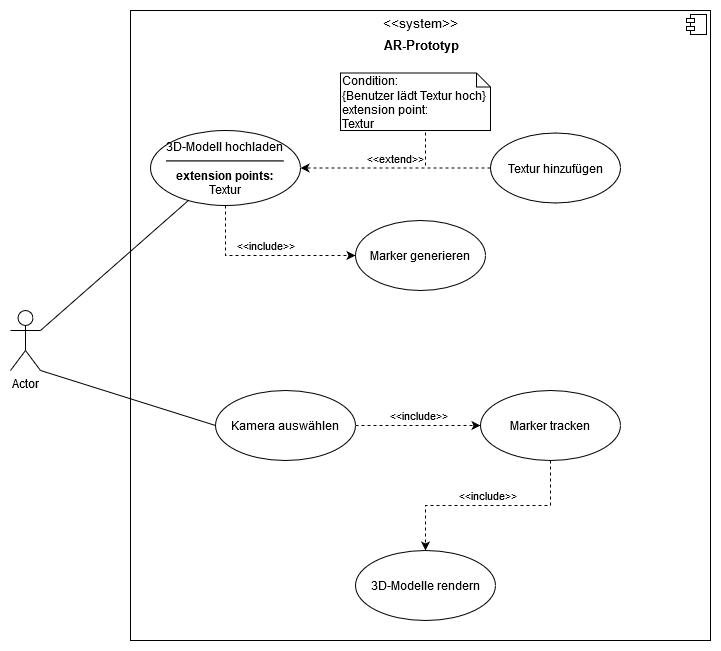
\includegraphics[width=1.0\textwidth]{Abbildungen/use-case-diagram.png}
\caption[Use Cases des Prototyps]{Use Case Diagramm des Prototyps. (Quelle: Eigene Darstellung)}
\label{fig:Use-Cases}
\end{figure}


\subsection{Anforderungsliste}
Im folgenden Abschnitt werden die Anforderungen an den Prototyp definiert. Dabei wird zwischen funktionalen und nichtfunktionalen Anforderungen unterschieden. \\
\begin{description}
\item[Funktionale Anforderungen] 
beschreiben die Funktionen eines Systemes, die notwendig sind, damit dieses seine Aufgaben erfüllen kann \citep[S. 10]{robertson:requirements-process}.
\item[Nichtfunktionale Anforderungen] 
beschreiben Eigenschaften, die das System besitzen muss, um den Nutzer zufrieden zustellen \citep[S. 10]{robertson:requirements-process}. Diese Eigenschaften beziehen sich vor allem auf die Bereiche Service Level, Zugriffsbeschränkungen, Sicherheit, Monitoring, Kontrolle, Schnittstellen, Archivierung, Benutzerfreundlichkeit und Konversion \citep[S. 139]{boehm:systementwicklung}
\end{description}
Die folgende Anforderungsliste leitet sich aus den ANwendungsfällen des Prototyps ab.

 
\subsubsection{Funktionale Anforderungen}
\begin{itemize}
\item[FA1] Die Anwendung soll ein Set von mindestens 10 Markern generieren können.
\item[FA2] Die Anwendung soll die generierten Marker in einem Kamerabild erkennen können.
\item[FA3] Die Anwendung soll die generierten Marker unterscheiden können.
\item[FA4] Der Benutzer soll eigene 3D-Modelle als OBJ-Dateien hochladen können.
\item[FA5] Die Anwendung soll OBJ-Datei laden und verarbeiten können.
\item[FA6] Die Anwendung soll Textur-Dateien im Bildformat(jpeg, png) laden und verarbeiten können.
\item[FA5] Die Anwendung soll den hochgeladenen Modellen einen generierten Marker zuordnen.
\item[FA6] Die Anwendung soll die 3D Modelle im Kamerabild anzeigen können.
\item[FA7] Die Anwendung soll die 3D-Modelle basierend auf der Transformation und Position der Marker im Kamerabild rendern.
\end{itemize}

\subsubsection{Nichtfunktionale Anforderungen}
\begin{itemize}
\item[NF1] Die Anwendung soll auf einem Android Smartphone(Huawei P30 Pro) laufen.
\begin{enumerate}
\item[NF1.1] Die Anwendung soll in Java mit Hilfe von Android Studio entwickelt werden.
\end{enumerate}

\item[NF2] Das Tracking soll mittels eines markerbasierten Verfahrens realisiert werden.
\item[NF3] Das Tracking soll mit 30FPS laufen.
\item[NF4] Das Tracking soll bei vollständig erkanntem Marker robust gegenüber Rotation, Skalierung, Perspektive und Belichtung sein.
\item[NF4] Die Anwednung soll ein simples User-Interface bereitstellen
\item[NF4] Mit Hilfe der UI soll ein Wechsel zwischen Kamera und Einstellungen möglich sein.
\item[NF4] Über die Einstellungsseite soll ein hochladen von 3D-Modellen möglich sein.

\end{itemize}

